\documentclass[12pt,addpoints]{repaso}
\grado{2}
\nivel{Secundaria}
\cicloescolar{2023-2024}
\materia{Ciencias y Tecnología: Física}
\unidad{3}
\title{Practica la Unidad}
\aprendizajes{
\item Describe la generación, diversidad y comportamiento de las ondas
    electromagnéticas como resultado de la interacción entre electricidad y
    magnetismo.
    \item Describe cómo se lleva a cabo la exploración de los cuerpos
    celestes por medio de la detección de las ondas electromagnéticas que emiten.
    \item Describe algunos avances en las características y composición del
    Universo (estrellas, galaxias y otros sistemas).
    \item Describe las características y dinámica del Sistema Solar.
    \item Identifica algunos aspectos sobre la evolución del Universo.
    }
\author{Melchor Pinto, J.C.}
\begin{document}
\INFO%
\begin{multicols}{2}
     \include*{../blocks/block006b}
     \include*{../blocks/block006c}
\end{multicols}
\begin{questions}
     \questionboxed[8]{\include*{../questions/question087a}}
     \newpage
     \questionboxed[8]{Relaciona cada enunciado con el concepto que le corresponda.

          \begin{multicols}{2}
               \begin{choices}\large
                    \choice Rayos X
                    \choice Luz visible
                    \choice Radiación infraroja
                    \choice Microondas
               \end{choices}

               \columnbreak%

               \begin{parts}\normalsize
                    \part \fillin[D][1cm] Poseen altas frecuencias y hacen vibrar las moléculas de agua, por lo que incrementan su temperatura.
                    \part \fillin[C][1cm] Es también conocida como radiación térmica, y es aplicada en la comunicación entre dispositivos electrónicos a corta distancia, como el control remoto de un televisor.
                    \part \fillin[B][1cm] Puede ser aprovechada por los seres vivos; por ejemplo, para generar energía química mediante la fotosíntesis.
                    \part \fillin[A][1cm] Poseen gran energía, por lo que pueden atravesar la materia blanda, pero no la dura.
               \end{parts}

          \end{multicols}

     }

     \ejemplosboxed[\include*{../questions/question076aaa}]

     \newpage

     \questionboxed[24]{\include*{../questions/question076a}}

     % \questionboxed[4]{\include*{../questions/question076b}}
     \ejemplosboxed[\include*{../questions/question085c}]

     \newpage

     \questionboxed[22]{\include*{../questions/question085d}}
     \newpage

     \normalsize

     \questionboxed[8]{Elige la respuesta correcta:

          \begin{multicols}{2}
               \begin{parts}
                    % \part ¿Cuál de las siguientes opciones describe la forma en que los astrónomos conciben al Universo según la teoría de la gran explosión?

                    % \begin{choices}
                    %     \choice El Universo es un fluido homogéneo y estático que siempre ha existido.
                    %     \choice El Universo es un fluido heterogéneo, estático y de inmensas proporciones.
                    %     \choice El Universo nació cuando la estrella primigenia agotó su combustible y explotó dando lugar a todo lo que existe.
                    %     \CorrectChoice El Universo es un fluido homogéneo y en expansión, constituido de radiación electromagnética y materia.
                    % \end{choices}


                    \part Antigüedad estimada del Universo.

                    \begin{choices}
                         \CorrectChoice 13,800 millones de años
                         \choice 18,300 millones de años
                         \choice 13,300 millones de años
                         \choice 11,800 millones de años
                    \end{choices}

                    \part Indica que el Universo se expande. %(pág. \pageref{086a_b})

                    \begin{choices}\normalsize
                         \choice El corrimiento al azul de la luz que emiten las galaxias.
                         \CorrectChoice El corrimiento al rojo de la luz que emiten las
                         galaxias.
                         \choice Todas las galaxias se alejan de la Vía Láctea.
                         \choice La Teoría de la Relatividad General
                    \end{choices}

                    \part La relación de proporcionalidad entre la velocidad con la que se
                    alejan las galaxias y la distancia a la que se encuentran.
                    %(pág. \pageref{086a_c})

                    \begin{choices}
                         \choice Ley de Hook
                         \choice Ley de Bubble
                         \CorrectChoice Ley de Hubble
                         \choice Ley de Moore
                    \end{choices}

                    \part Longitud del diámetro del Universo.

                    \begin{choices}
                         \choice Un millón de años luz.
                         \CorrectChoice Cien mil millones de años luz.
                         \choice Mil millones de años luz.
                         \choice Un billón de años luz.

                    \end{choices}

                    % \part Pulso eléctrico que se propaga a través de la neurona.

                    % \begin{choices}
                    %     \CorrectChoice Potencial de acción
                    %     \choice Potencial eléctrico
                    %     \choice Potencial magnético
                    %     \choice Energía potencial
                    % \end{choices}

                    % \part Perturbación eléctrica que se genera cuando una neurona recibe un estímulo.

                    % \begin{choices}
                    %     \choice Impulso eléctrico
                    %     \CorrectChoice Impulso nervioso
                    %     \choice Impulso magnético
                    %     \choice Impulso atómico
                    % \end{choices}


               \end{parts}
          \end{multicols}
     }

     \questionboxed[10]{Señala si son verdaderas o falsas las siguientes afirmaciones.
          \begin{multicols}{2}

               \begin{parts}
                    % \part Cuando se viaja de norte a sur, o viceversa, la altura aparente de las estrellas cambia.

                    % \begin{oneparchoices}
                    %     \CorrectChoice Verdadero
                    %     \choice Falso
                    % \end{oneparchoices}



                    \part La Tierra no rota sobre su propio eje porque nosotros no percibimos que nos estamos moviendo.

                    \begin{oneparchoices}
                         \choice Verdadero
                         \CorrectChoice Falso
                    \end{oneparchoices}



                    % \part En la siguiente imagen se puede apreciar, mediante el ordenamiento de las limaduras de hierro, el campo magnético de los polos iguales de dos imanes.

                    % \begin{oneparchoices}
                    %     \choice Verdadero
                    %     \choice Falso
                    % \end{oneparchoices}\hfill
                    % 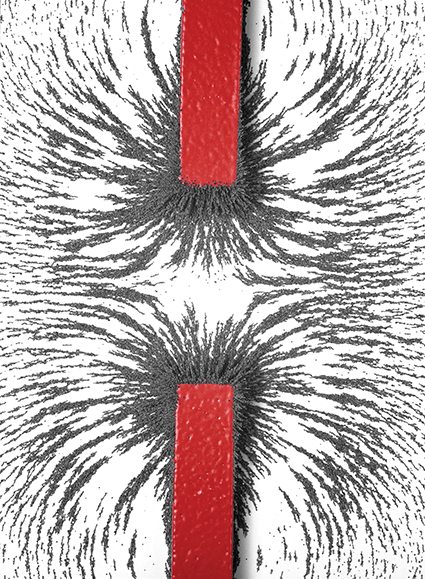
\includegraphics[width=0.3\linewidth]{SINFI_U2_AC67_IMGS4.jpg}




                    \part El hecho de que en el mar primero desaparece el casco y luego la vela de un navío es un argumento sobre la redondez de la Tierra.

                    \begin{oneparchoices}
                         \CorrectChoice Verdadero
                         \choice Falso
                    \end{oneparchoices}

                    \part Toda carga en movimiento genera un campo magnético.

                    \begin{oneparchoices}
                         \choice Verdadero
                         \choice Falso
                    \end{oneparchoices}

                    \part La fuerza magnética es una interacción de acción a distancia, también llamada fuerza de campo.

                    \begin{oneparchoices}
                         \choice Verdadero
                         \choice Falso
                    \end{oneparchoices}

                    \part Cuando acercamos dos imanes por sus polos iguales, los campos magnéticos interactúan y se suman, de tal forma que los imanes experimentan una fuerza de atracción mutua.

                    \begin{oneparchoices}
                         \choice Verdadero
                         \choice Falso
                    \end{oneparchoices}

                    \part Sólo las cargas masivas producen campos magnéticos.

                    \begin{oneparchoices}
                         \choice Verdadero
                         \choice Falso
                    \end{oneparchoices}

                    \part En un eclipse solar se observa que la Luna pasa delante del Sol y que ambos tienen un tamaño en apariencia iguales.
                    De ello se concluye que el Sol está a la misma distancia que la Luna.

                    \begin{oneparchoices}
                         \choice Verdadero
                         \CorrectChoice Falso
                    \end{oneparchoices}
                    % \part Los electrones que orbitan alrededor del núcleo generan corrientes eléctricas que, a su vez, producen campos magnéticos, por lo que los átomos se comportan como imanes.

                    % \begin{oneparchoices}
                    %     \choice Verdadero
                    %     \choice Falso
                    % \end{oneparchoices}

                    % \part En la siguiente figura, la flecha azul indica la dirección del campo magnético.

                    % 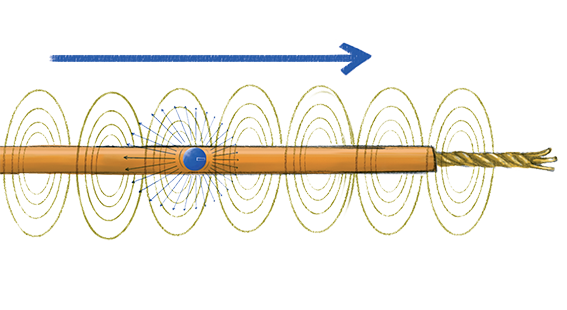
\includegraphics[width=\linewidth]{SINFI_U2_AC67_IMGS2.png}

                    % \begin{oneparchoices}
                    %     \choice Verdadero
                    %     \choice Falso
                    % \end{oneparchoices}\hfill


                    % \part La siguiente figura ilustra el ordenamiento de los “imanes atómicos” de un material magnético.

                    % 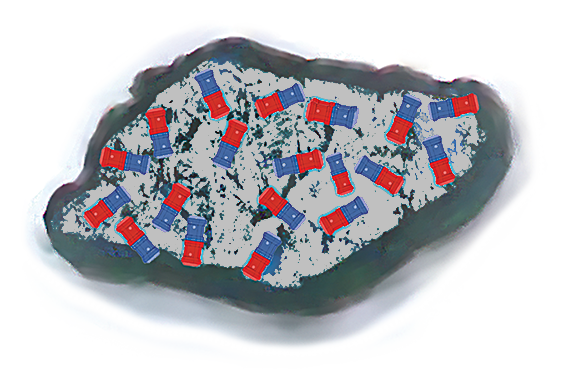
\includegraphics[width=0.5\linewidth]{SINFI_U2_AC67_IMGS3.png}

                    % \begin{oneparchoices}
                    %     \choice Verdadero
                    %     \choice Falso
                    % \end{oneparchoices}

                    \part La Tierra posee un campo magnético debido a las corrientes internas en su núcleo de hierro fundido.

                    \begin{oneparchoices}
                         \choice Verdadero
                         \choice Falso
                    \end{oneparchoices}



                    \part La dirección del campo magnético de un conductor largo y recto por el que circula una corriente es circular y rodea al alambre.

                    \begin{oneparchoices}
                         \choice Verdadero
                         \choice Falso
                    \end{oneparchoices}


                    \part La sombra que la Tierra proyecta sobre la Luna en los eclipses lunares es un argumento sobre la redondez de la Tierra.

                    \begin{oneparchoices}
                         \CorrectChoice Verdadero
                         \choice Falso
                    \end{oneparchoices}
               \end{parts}
          \end{multicols}
     }


     \questionboxed[20]{Selecciona la respuesta correcta:

          \begin{multicols}{2}
               \begin{parts}


                    \part Porcentaje de energía oscura que hay en el Universo.

                    \begin{oneparchoices}
                         \choice 4.9\%
                         \choice 26.8\% \\
                         \choice 33.3\%
                         \CorrectChoice 68.3\%
                    \end{oneparchoices}

                    \part Células receptoras de luz capaces de percibir colores, pero para que funcionen es necesario que haya suficiente luz.

                    \begin{oneparchoices}
                         \choice Bastones
                         \choice Esferas \\
                         \CorrectChoice Conos
                         \choice Rizos
                    \end{oneparchoices}

                    \part Porcentaje de materia ordinaria que hay en el Universo.

                    \begin{oneparchoices}
                         \CorrectChoice 4.9\%
                         \choice 26.8\% \\
                         \choice 33.3\%
                         \choice 68.3\%
                    \end{oneparchoices}

                    \part Es un sistema de estrellas, gas y polvo interestelar que orbita en torno a un centro de gravedad. %(pág. \pageref{085a_a})

                    \begin{oneparchoices}
                         \choice Cúmulo
                         \CorrectChoice Galaxia \\
                         \choice Nebulosa
                         \choice Pulsar
                    \end{oneparchoices}

                    % \part Unidad conveniente para medir el tamaño de las galaxias. %(pág. \pageref{085a_b})

                    % \begin{oneparchoices}
                    %     \choice Metro
                    %     \choice Millas aéreas \\
                    %     \choice Kilómetro
                    %     \CorrectChoice Año Luz
                    % \end{oneparchoices}

                    \part Variación aparente de la posición de un objeto al cambiar la posición del observador.

                    \begin{oneparchoices}
                         \choice Eclipse
                         \choice Declinación \\
                         \choice Transformación
                         \CorrectChoice Paralaje
                    \end{oneparchoices}

                    \part Es la magnitud que mide un año luz. %(pág. \pageref{085a_c})

                    \begin{oneparchoices}
                         \choice Tiempo
                         \choice Masa \\
                         \CorrectChoice Longitud
                         \choice Energía
                    \end{oneparchoices}

                    \part Número aproximado de galaxias en el Universo.%(pág. \pageref{085a_d})

                    \begin{oneparchoices}
                         \choice miles
                         \CorrectChoice billones \\
                         \choice millones
                         \choice trillones
                    \end{oneparchoices}

                    \part Proporción detectable de una galaxia por medio de las ondas electromagnéticas. %(pág. \pageref{085a_e})

                    \begin{oneparchoices}
                         \CorrectChoice 10\%
                         \choice 20\% \\
                         \choice 30\%
                         \choice 40\%
                    \end{oneparchoices}

                    % \part Masa que no es detectable por medio de las ondas electromagnéticas de la cual se conoce su existencia
                    % por la manera en que afecta a la rotación de las estrellas más alejadas del núcleo galáctico.% (pág. \pageref{085a_f})

                    % \begin{oneparchoices}
                    %     \choice Energía oscura
                    %     \CorrectChoice Materia oscura
                    %     \choice Fuerza oscura
                    %     \choice Masa oscura
                    % \end{oneparchoices}

                    % \part Instrumento gracias al cual es posible observar cuerpos celestes muy lejanos.

                    % \begin{oneparchoices}
                    %     \choice Microscopio
                    %     \choice Estetoscopio \\
                    %     \CorrectChoice Telescopio
                    %     \choice Electroscopio
                    % \end{oneparchoices}

                    \part Porcentaje de materia oscura que hay en el Universo.

                    \begin{oneparchoices}
                         \choice 4.9\%
                         \CorrectChoice 26.8\% \\
                         \choice 33.3\%
                         \choice 68.3\%
                    \end{oneparchoices}


                    % \part Aparato que sirve para medir ángulos muy pequeños que ayudó a medir la distancia a la cual se encuentran algunos objetos celestes.

                    % \begin{oneparchoices}
                    %     \choice Vernier
                    %     \choice Micrómetro \\
                    %     \CorrectChoice Astrolabio
                    %     \choice Transportador
                    % \end{oneparchoices}

                    \part Técnica gracias a la cual se puede comparar el cambio en la posición de una estrella al transcurrir cierto período de tiempo.

                    \begin{oneparchoices}
                         \choice Radiografía
                         \choice Radiometría \\
                         \CorrectChoice Fotografía
                         \choice Espectroscopía
                    \end{oneparchoices}



               \end{parts}
          \end{multicols}
     }

     % \newpage


     % \questionboxed[4] \include*{../questions/question077a}


     % \newpage
     % \questionboxed[10] \include*{../questions/question088b}


     % \newpage
     % \questionboxed[10] \include*{../questions/question090a}
     % \questionboxed[10] \include*{../questions/question089b}
     % \newpage
     % \questionboxed[10] \include*{../questions/question087c}
     % \questionboxed[15] \include*{../questions/question085c}
\end{questions}
\end{document}
